%&"pre"
% \endofdump
% \tikzexternalize[prefix=cache/]{b4paperreading}
\begin{document}
    \title{B4: Google's Software-Defined WAN}
    \subtitle{Paper Reading}
    \author{Log Creative}
    \date{\today}
    \maketitle

    \begin{frame}
        \frametitle{论文}
        \fullcite{Hong2018}
    \end{frame}

    \section{简介}

    \begin{frame}
        \frametitle{B4}
        \framesubtitle{Google 私有广域网后端}
        \framezoom<1><2>(1cm,1.5cm)(3cm,2cm)
        \begin{figure}
            \centering
            \includegraphics[height=0.6\textheight]{b4.pdf}
            \caption{B4 全球网络}
        \end{figure}
        \only<2>{
            \begin{tikzpicture}[overlay]
                \node [right] at (1cm,4cm) {TE};
                \node [right] at (1cm,3.7cm) {\tiny Traffic};
                \node [right] at (1cm,3.5cm) {\tiny Engineering};
            \end{tikzpicture}
        }
    \end{frame}

    \begin{frame}
        \frametitle{SLO}
        \framesubtitle{Service Level Objectives 服务级别协议}
        表示 30 天滑动窗口内的网络连接可用性和带宽可用性。
        \begin{table}
            \begin{tabular}{clr}
                \toprule
                服务级别 & 应用举例 & SLO需求\\
                \midrule
                \rowcolor<3>{csecondary!30} SC4 & 搜索广告、DNS、WWW & 99.99\%\\
                SC3 & 照片服务后端、邮件 & 99.95\%\\
                SC2 & 广告数据库拷贝 & 99.90\%\\
                SC1 & 搜索索引拷贝 & 99\%\\
                \rowcolor<2>{ctertiary!30} SC0 & 批量传输 & \\
                \bottomrule
            \end{tabular}
            \caption{SLO}
        \end{table}
    \end{frame}

    \section{背景与动机}

    \begin{frame}
        \frametitle{扁平结构}
        \framesubtitle{不利于扩展和可用性}
        之前的 B4 若想增加容量,需要在地理限界内增加站点。但这会带来:
        \begin{enumerate}
            \item 增加了中央流量控制优化算法的运行时间。
            \item 对交换机有限的流表空间增加压力。
            \item 使得容量管理变得复杂并给应用开发者造成麻烦。
        \end{enumerate}
        \only<2>{为了解决这个问题,引入 \emph{supernode}(超级节点)和两层架构。} % 后文讨论细节
    \end{frame}

    \begin{frame}
        \frametitle{分层架构}
        \framesubtitle{容量不对等问题}
        B4 中 6--20\% 的地理级连接仍然会在 $\geq$ 5\% 的时间内有容量不对等情形。
        \begin{figure}[H]
            \centering
            \includegraphics[height=0.5\textheight]{asym}

            $\frac{\text{avg}_{\forall i} C_i - \text{min}_{\forall i} C_i}{\text{avg}_{\forall i} C_i}$
            \caption{地理级流量不对等}\label{fig:asym}
        \end{figure}
    \end{frame}

    \begin{frame}[label=asym]
        \frametitle{不对等的后果}
        \framesubtitle{大幅减少系统效率}

        \begin{figure}
        \centering
        \begin{tikzpicture}
            \tikzstyle{supernode}=[rectangle,draw,minimum width=1.5cm,minimum height=1cm,fill=white];
            \tikzstyle{flow}=[->];
            \draw[draw=none,fill=cprimary!10]  (-1.5,2) rectangle (0.5,-2);
            \draw[draw=none,fill=cprimary!10]  (1.5,2) rectangle (3.5,-2);
            \node[supernode] (a1) at (-0.5,1) {$A_1$};
            \node [supernode] (b1) at (2.5,1) {$B_1$};
            \node [supernode] (b2) at (2.5,-1) {$B_2$};
            \only<1,3>{
                \node [supernode] (a2) at (-0.5,-1) {$A_2$};
                \draw [flow](-2,-1) node[left]{$\frac{c}{2}$} -- (a2);
            }
            \only<2>{
                \node [supernode,draw=csecondary] (a2) at (-0.5,-1) {\color{csecondary}$A_2$};
                \draw [flow,csecondary](-2,-1) node[left]{\color{csecondary} $\frac{c}{2}$} -- (a2);
            }
            \node at (-0.5,2.5) {Site $A$};
            \node at (2.5,2.5) {Site $B$};
            \draw[flow] (-2,1) node[left] {$\frac{c}{2}$} -- (a1);
            
            \draw (a1) -- (b2);
            \draw  (a1) edge (b1);
            \only<1>{
                \draw (a2) edge node[above] {5} (b1);
                \draw (a2) edge node[above] {5} (b2);
            }
            \only<2->{
                \draw[csecondary] (a2) edge node[above] {1} (b1);
                \draw[csecondary]  (a2) edge node[above] {1} (b2);
            }
            \draw  (b1) edge node [right] {4} (b2);
            \only<3->{
                \draw[cprimary] (a1) edge node [left] {\emph{sidelink}} node[right] {4} (a2);
            }
        \end{tikzpicture}
        \caption{\only<1>{对等} \only<2->{不对等示例} \only<2>{$c=4$} \only<3>{$c=12$}}\label{fig:asymeg}
        \end{figure}
    \end{frame}

    \begin{frame}
        使用 \emph{sidelink} 可以提高不对等时的带宽利用率。但是仍然需要考虑相关的协议问题,比如有些数据不可分割、MAC 地址不可变化,% 后文使用算法解决。
        
        以及死循环问题,转换隧道可能是\emph{原子操作},以任意顺序应用 TE 更新会导致这种死循环率上升,% 后文会通过另一种算法完成。
    \end{frame}

    \begin{frame}
        \frametitle{高效交换规则管理}
        Merchant 交换机只支持有限的匹配和哈希规则。

        % 后文补充
    \end{frame}

    \section{站点拓扑的进化}

    % \begin{frame}
    %     \frametitle{站点拓扑演化}
    %     \begin{table}
    %         \centering
    %         \includegraphics[width=\linewidth]{gentable}
    %         \caption{B4 结构世代}\label{tab:gentable}
    %     \end{table}
    % \end{frame}

    \begin{frame}
        \frametitle{Saturn}
        \framesubtitle{第一代 B4 网络结构}
        \begin{columns}
            \begin{column}{0.4\textwidth}
                \begin{figure}
                    \includegraphics[width=\linewidth]{saturn}
                    \caption{Saturn 站点}
                \end{figure}
            \end{column}
            \begin{column}{0.6\textwidth}
                \begin{table}
                    \begin{tabular}{>{\bfseries}ll}
                        \toprule
                        名称 & Saturn \\
                        部署年 & 2010 \\
                        类型 & 数据中心 \\
                        交换机芯片 & 24x10G \\
                        每站点机箱数 & 6 / 8 \\
                        站点容量 (Tbps) & 5.12 \textsc{ex} 2.56 \textsc{inter}\\
                        每站点交换机箱数 & 4 \\
                        控制域数量 & 1 \\
                        \bottomrule
                    \end{tabular}
                    \caption{Saturn 站点}\label{tab:saturn}
                \end{table}
            \end{column}
        \end{columns}
    \end{frame}

    \begin{frame}
        \frametitle{Jumpgate: JPOP}
        \framesubtitle{仅传输站点}
        \begin{columns}
            \begin{column}{0.4\textwidth}
                \begin{figure}
                    \includegraphics[height=0.7\textheight]{jpop}
                    \caption{JPOP 站点}
                \end{figure}
            \end{column}
            \begin{column}{0.6\textwidth}
                \begin{table}
                    \begin{tabular}{>{\bfseries}ll}
                        \toprule
                        名称 & JPOP \\
                        部署年 & 2013 \\
                        类型 & POP \\
                        交换机芯片 & 16x40G \\
                        每站点机箱数 & 20 \\
                        超级节点交换机数 & 24 \\
                        站点容量 (Tbps) & 10.24\\
                        每站点交换机箱数 & 4 \\
                        控制域数量 & 2 \\
                        \bottomrule
                    \end{tabular}
                    \caption{JPOP 站点}\label{tab:jpop}
                \end{table}
            \end{column}
        \end{columns}
    \end{frame}

    \begin{frame}
        \frametitle{Jumpgate: Stargate}
        \framesubtitle{数据中心级}
        \begin{columns}
            \begin{column}{0.4\textwidth}
                \begin{figure}
                    \includegraphics[height=0.7\textheight]{stargate}
                    \caption{Stargate 站点}
                \end{figure}
            \end{column}
            \begin{column}{0.6\textwidth}
                \begin{table}
                    \begin{tabular}{>{\bfseries}ll}
                        \toprule
                        名称 & Stargate \\
                        部署年 & 2014 \\
                        类型 & 数据中心 \\
                        交换机芯片 & 32x40G \\
                        每站点机箱数 & 192 \\
                        超级节点交换机数 & 48 \\
                        站点容量 (Tbps) & 81.92\\
                        每站点交换机箱数 & 8 \\
                        控制域数量 & 4 \\
                        \bottomrule
                    \end{tabular}
                    \caption{Stargate 站点}\label{tab:stargate}
                \end{table}
            \end{column}
        \end{columns}
    \end{frame}

    \begin{frame}
        \frametitle{Jumpgate: Stargate}
        \framesubtitle{数据吞吐量大带来的好处}

        \begin{columns}
            \begin{column}{0.2\textwidth}
                \begin{figure}
                    \includegraphics[width=\linewidth]{stargateswitch}
                    \caption{交换机与交换机架}
                \end{figure}
            \end{column}
            \begin{column}{0.6\textwidth}
                \begin{figure}
                    \includegraphics[width=\linewidth]{stargatesubsumes}
                    \caption{减少 BGP 复杂度}
                \end{figure}
            \end{column}
        \end{columns}
    \end{frame}

    \section{分层流量工程}

    \begin{frame}
        \frametitle{简单粗暴的提案}
        \framesubtitle{平面流量工程}
        \highlight[csecondary]{方法}~直接对站点内所有的超级节点直接应用流量控制。这种模型下,由一个中央控制器使用 IP-in-IP 封装对超级节点级隧道进行负载均衡。

        \paragraph{缺点} 高运行时间、花费大量的交换机流表空间、不可扩展。每个站点内有4个超级节点,那么站点到站点间的3跳转发会有$4^3=64$条路径。
    \end{frame}

    \begin{frame}
        \frametitle{简单粗暴的提案}
        \framesubtitle{最短路转发}

        \highlight[csecondary]{方法}~超级节点级链路实现最短路转发。

        \paragraph{优点}拥有扩展性、只需要一层封装、在广域网失效时能够通过\alert{旁路链接}完成流量转移。

        \paragraph{缺点}无法处理容量不对等情形,不是完全失效的情况下无法找到通过\alert{旁路链接}得到的更长但容量更大的路径。
        \hyperlink{asym<3>}{\beamergotobutton{不对等的后果}}
    \end{frame}

    \begin{frame}
        \frametitle{分层流量工程结构}
        \framesubtitle{概念}
        \begin{columns}
            \begin{column}{0.6\textwidth}
                \begin{itemize}
                    \item[SSG] \emph{Switch Split Group} 确定物理交换机所分割的流量。
                    \item[TSG] \emph{Tunnel Split Group} 确定一个链路\emph{tunnel}内如何分配两个站点超级节点间的流量分布。
                    \item[TG] \emph{Tunnel Group} 通过 IP-in-IP 封装映射 FG 到一个链路集合。 
                    \item[FG] \emph{Flow Group} $\langle$源站点, 目标站点, 服务类别$\rangle$ 
                \end{itemize}
            \end{column}
            \begin{column}{0.4\textwidth}
                \begin{figure}
                    \centering
                    \includegraphics[width=0.9\linewidth]{hitearch}
                    \caption{不同的流量工程结构}
                \end{figure}
            \end{column}
        \end{columns}
    \end{frame}

    \begin{frame}
        \frametitle{分层流量工程结构}
        \framesubtitle{运行概览}
        \begin{algorithm}[H]
            \caption{B4 运行概览}
            域控制器通过聚合可用的物理链路容量来计算超级节点间的连接\;
            中央控制器根据上述结果计算 TSG 来分配每一条站点级的出口连接\;
            \leIf{对等}{不使用旁路连接\;}{通过旁路连接重新分配TSG}
            使用上述 TSG 结果计算站点级每条链路的有效容量,生成 TG\;
            生成 TE 操作的无环依赖图\;
            通过生成 SSG 分割规则,按照次序对 FG, TG, TSG 编程\;
        \end{algorithm}
    \end{frame}

    \begin{frame}
        \frametitle{TSG 生成算法}
        \framesubtitle{问题描述}
        假设进入隧道的流量对于源站点的所有超级节点来说都是平均分割的。对于沿着隧道的每个站点内的每一个超级节点计算 TSG,使得能够最大化利用对应超级节点连接容量的上限。使用正整数表示输出链路上的每一连接的相对权重,并要求每一个 TSG 的权重总和不能超过一个阈值 $T$,因为交换器哈希表键值数量限制。
    \end{frame}

    \begin{frame}
        \frametitle{TSG 生成算法}
        \framesubtitle{例子\only<4->{(罕见)}}
        \begin{figure}
            \centering
            \begin{tikzpicture}
                \tikzstyle{supernode}=[rectangle,draw,minimum width=1cm,minimum height=0.7cm,fill=white];
                \tikzstyle{flow}=[->, line width=1pt];
                \node [supernode] (a1) at (-1.5,1.5) {$A_1$};
                \node [supernode] (a2) at (-1.5,-0.5) {$A_2$};
                \node [supernode] (b1) at (1,1.5) {$B_1$};
                \node [supernode] (b2) at (1,-0.5) {$B_2$};
                \node [supernode] (c1) at (3.5,1.5) {$C_1$};
                \node [supernode] (c2) at (3.5,-0.5) {$C_2$};
                \only<1-4>{
                    \draw  (a1) edge (a2);
                }
                \only<5,6>{
                    \draw [flow] (a2) edge node [right] {\only<5>{$3c/8$}\only<6>{$c/2$}} (a1);
                }
                \draw  (c1) edge (c2);
                \path [flow] (-3,1.5) edge node[above] {\only<1>{$2c$}\only<2,4>{$c$}\only<3>{$1.5c$}\only<5>{$9c/8$}} (a1);
                \path [flow] (-3,-0.5)  edge node[above] {\only<1>{$2c$}\only<2,4>{$c$}\only<3>{$1.5c$}\only<5>{$9c/8$}} (a2);
                \only<1-3,5,6>{
                    \draw [flow] (a1) edge node [above,sloped] {\only<1,6>{$c$}\only<2>{$0.5c$}\only<3>{$0.75c$}\only<5>{$6c/8$}} (b1);
                    \draw [flow] (a2) edge node [above,sloped] {\only<1,6>{$c$}\only<2>{$0.5c$}\only<3>{$0.75c$}\only<5>{$6c/8$}} (b1);
                }
                \only<4>{
                    \draw (a1) edge (b1);
                    \draw (a2) edge (b1);
                }
                \draw [flow] (a1) edge node [above,sloped] {\only<1,4,6>{$c$}\only<2>{$0.5c$}\only<3>{$0.75c$}\only<5>{$6c/8$}} (b2);
                \only<1-4>{
                    \draw [flow] (a2) edge node [above,sloped] {\only<1,4>{$c$}\only<2>{$0.5c$}\only<3>{$0.75c$}} (b2);
                }
                \only<5,6>{
                    \draw [dashed] (a2) edge (b2);
                }
                \only<1>{
                    \draw [flow] (b1) edge node [above,sloped] {$c$} (c1);
                    \draw [flow] (b1) edge node [above,sloped] {$c$} (c2);
                    \draw  (b2) edge (b1);
                }
                \only<2>{
                    \draw [dashed] (b1) edge (c1);
                    \draw [dashed] (b1) edge (c2);
                    \draw [flow] (b1) edge node [right] {$c$} (b2);
                }
                \only<3,5,6>{
                    \draw [dashed] (b1) edge (c1);
                    \draw [flow] (b1) edge node [above,sloped] {$c$} (c2);
                    \draw [flow] (b1) edge node [right] {\only<3>{$0.5c$}\only<5>{$4c/8$}\only<6>{$c$}} (b2);
                }
                \only<4>{
                    \draw [dashed] (b1) edge (c1);
                    \draw [dashed] (b1) edge (c2);
                    \draw [dashed] (b1) edge (b2);
                }
                \draw [flow] (b2) edge node [above,sloped] {\only<1-4,6>{$c$}\only<5>{$5c/8$}} (c1);
                \draw [flow] (b2) edge node [above,sloped] {\only<1-4,6>{$c$}\only<5>{$5c/8$}} (c2);
                \path [flow] (c1)  edge node[above] {\only<1>{$2c$}\only<2,4>{$c$}\only<3>{$c$}\only<5>{$5c/8$}\only<6>{$c$}}  (5,1.5);
                \path [flow] (c2)  edge node[above] {\only<1>{$2c$}\only<2,4>{$c$}\only<3>{$2c$}\only<5>{$13c/8$}\only<6>{$2c$}}  (5,-0.5);
            \end{tikzpicture}
            \caption{
                \only<1>{对等网络 $TC=4c$}
                \only<2>{不对等网络 $TC=2c$}
                \only<3>{不对等网络 $TC=3c$}
                \only<4>{$TC=0$ ($B_1$故障) 或 $TC=2c$ ($B_1$关闭)}
                \only<5>{$TC=9c/4$ (次优解)}
                \only<6>{$TC=3c$ (最优解)}
            }
        \end{figure}
    \end{frame}

    \makebottom
\end{document}